% Chapter Chapter 3 For Reproducible Research in R and RStudio
% Christopher Gandrud
% Created: 16/07/2012 05:45:03 pm CEST
% Updated: 4 September 2012




\chapter{Getting Started with R, RStudio, and knitr}\label{GettingStarted}

If you have rarely or never used R before the first two sections of this chapter give you enough information to be able to get started and understand the code I use in this book. For more detailed introductions to R please refer to the related resources I mentioned in chapter \ref{WhatNot}. Experienced R users might want to skip the first two sections of the chapter. This chapter also gives a brief overview of RStudio. It highlights the key features of main RStudio panel (what appears when you open RStudio) and some of its key features for reproducible research. Finally, I discuss the basics of the {\emph{knitr}} package and how it is integrated into RStudio.

%%%%%%%%%%%%% Using R
\section{Using R: the basics}

As a computer language, R has FILL in

This section covers some of the very basic syntax in R to get you started. If you have little experience with R, reading this section will make it much easier for you to follow along with the examples in the book. I cover the key components of the R language including:

\begin{itemize}
    \item objects \& assignment,
    \item component selection,
    \item functions, commands, and arguments,
    \item libraries.
\end{itemize}

Before discussing each of these components let's open up R and look around.\footnote{Please see Chapter \ref{Intro} for instructions on how to install R.} When you open up R you should get a window that looks something like what you see in Figure \ref{RBlankMain}.\footnote{This figure and almost all screenshots in this book are from a computer using the Mac OS 10.8 operating system.} This window is the {\bf{R console}}\index{R console}. Under the session\index{session information} information--what version of R you are using, your workspace, and so on--you should see a {\tt{\textgreater}}. This is where you enter R code.\footnote{If you are using a Unix-like system such as Ubuntu or Mac OS 10, you can an application called the Terminal\index{Terminal}. If you have installed R on your computer you can type {\tt{r}} into the terminal and then the {\tt{Enter}} or {\tt{Return}} key it will begin a new R session. You know if a new R session has started if you get the same startup information is printed in the Terminal window.} To run R code that you have typed into the console type the {\tt{Enter}} or {\tt{Return}} key. Now that we have a new R session open we can get started. 

\begin{figure}[th!]
    \caption{R Startup Console}
    \label{RBlankMain}
    \begin{center}
    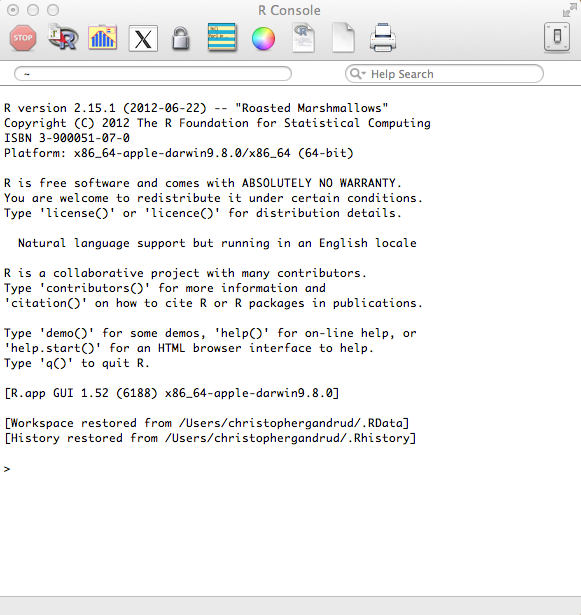
\includegraphics[scale=0.4]{/git_repositories/Rep-Res-Book/Source/Children/Chapter3/images3/BlankRConsole.png}
    \end{center}
\end{figure}

\subsection{Objects}

You will probably have read that `R is an object-oriented\index{object-oriented} language'.  What are objects? Objects are like the R language's nouns. They are things, such as a list of numbers, a data set, a word, a table of results from some analysis, and so on. Saying that R is `object-oriented' just means that R is focused on doing actions to objects. We will talk about the actions--commands and functions--later in this section. For now let's create a few objects.

\paragraph{Numeric \& string objects}

Different types of objects have different data types or modes\index{mode}. Let's make two basic objects of the numeric and character mode. We can choose almost any name we want for our objects.\footnote{Objects must begin with an alphabetic character and cannot have spaces.} Let's call our numeric object {\emph{Number}}. To put something into the object we use the {\bf{assignment operator}}: {\tt{\textless -}}. Let's assign the number 10 to our Number object.

\begin{knitrout}
\definecolor{shadecolor}{rgb}{0.969, 0.969, 0.969}\color{fgcolor}\begin{kframe}
\begin{alltt}
Number <- 10
\end{alltt}
\end{kframe}
\end{knitrout}


\noindent To see the contents of our object, just type its name.

\begin{knitrout}
\definecolor{shadecolor}{rgb}{0.969, 0.969, 0.969}\color{fgcolor}\begin{kframe}
\begin{alltt}
Number
\end{alltt}
\begin{verbatim}
## [1] 10
\end{verbatim}
\end{kframe}
\end{knitrout}


\noindent Lets's briefly breakdown this output. \texttt{10} is clearly the contents of {\emph{Number}}. The double hash (\texttt{\#\#}) is included in the output by {\emph{knitr}} to tell you that this is output rather than R code.\footnote{This makes it easier to copy and past code included in a presentation document by {\emph{knitr}}.} Finally, \texttt{[1]} is the row number of the object that 10 is on. Clearly our object only has one row.   

Creating a character object is very similar. The only difference is that we enclose the character string (letters in a word for example) inside of quotation marks ({\tt{""}}). To create an object called {\emph{Words}} that contains a character string ``Hello World".

\begin{knitrout}
\definecolor{shadecolor}{rgb}{0.969, 0.969, 0.969}\color{fgcolor}\begin{kframe}
\begin{alltt}
Words <- \hlstring{"Hello World"}
\end{alltt}
\end{kframe}
\end{knitrout}



An object's class is important to keep in mind as it determines what things we can do to it. For example you cannot take the mean of a character mode object like the {\emph{Words}} object we created earlier:

\begin{knitrout}
\definecolor{shadecolor}{rgb}{0.969, 0.969, 0.969}\color{fgcolor}\begin{kframe}
\begin{alltt}
\hlfunctioncall{mean}(Words)
\end{alltt}


{\ttfamily\noindent\textcolor{warningcolor}{\#\# Warning: argument is not numeric or logical: returning NA}}\begin{verbatim}
## [1] NA
\end{verbatim}
\end{kframe}
\end{knitrout}


\noindent Trying to find the mean of our {\emph{Words}} object gave us a warning message and returned the value {\tt{NA}}\index{NA}: not applicable. You can also think of {\tt{NA}} to mean missing. To find out what class an object has use the {\tt{class}} command. For example:

\begin{knitrout}
\definecolor{shadecolor}{rgb}{0.969, 0.969, 0.969}\color{fgcolor}\begin{kframe}
\begin{alltt}
\hlfunctioncall{class}(Words)
\end{alltt}
\begin{verbatim}
## [1] "character"
\end{verbatim}
\end{kframe}
\end{knitrout}


\paragraph{Vector \& data frame objects}

Sp far we have only looked at objects with a single number or string.\footnote{These might be called scalar objects, though in R scalars are just vectors with a length of 1.} Clearly we want to be using objects--data sets--that have many strings and numbers. In R these are usually {\bf{data frame}}\index{data frame} type objects and are roughly equivalent to the type of data structure you would be familiar with from using a program such as Microsoft Excel. We will be using data frames extensively throughout the book. It is also useful to cover other, simpler types of objects, primarily vectors. Vectors are R's ``workhorse".\cite{Matloff2011} Knowing how to use vectors\index{vector} will be especially helpful when we clean up raw data in Chapter \ref{DataClean} and make tables in Chapter \ref{TablesChapter}.\footnote{If you want information about other types of R objects such as lists\index{list} and matrices\index{matrix}, Chapter 1 of Norman Matloff's book\cite{Matlof2011} is a really good place to look.} \\[0.25cm]

\noindent {\bf{Vectors}}: \\[0.25cm] Vectors are the ``fundamental data type"\cite{Matloff2011} in R. They are simply an ordered group of numbers, character strings, and so on.\footnote{In a vector every member of the group must be of the same type. Lists are similar to vectors, but allow you to have different types.} It may be useful to think of basically all other data types as complicated forms of vectors. For example, data frames are basically multiple vectors of the same length--i.e. they have the same number of rows--and possibly of different types attached together. 

Let's create a very simple numeric vector containing the numbers 2.8, 2, and 14.8. To do this we will use the \texttt{c} (concatenate)\index{concatenate} function:

\begin{knitrout}
\definecolor{shadecolor}{rgb}{0.969, 0.969, 0.969}\color{fgcolor}\begin{kframe}
\begin{alltt}
NumericVect <- \hlfunctioncall{c}(2.8, 2, 14.8)

\hlcomment{# Show NumericVect's contents}
NumericVect
\end{alltt}
\begin{verbatim}
## [1]  2.8  2.0 14.8
\end{verbatim}
\end{kframe}
\end{knitrout}


Vectors of character strings are created in a similar way. The only major difference is that each character string is enclosed in quotation marks like this:

\begin{knitrout}
\definecolor{shadecolor}{rgb}{0.969, 0.969, 0.969}\color{fgcolor}\begin{kframe}
\begin{alltt}
CharacterVect <- \hlfunctioncall{c}(\hlstring{"Albania"}, \hlstring{"Botswana"}, \hlstring{"Cambodia"})

\hlcomment{# Show CharacterVect's contents}
CharacterVect
\end{alltt}
\begin{verbatim}
## [1] "Albania"  "Botswana" "Cambodia"
\end{verbatim}
\end{kframe}
\end{knitrout}


To give you a preview of what we are going to do when we start working with real data sets, lets combine the two vectors {\emph{NumericVect}} and {\emph{CharacterVect}} into a new object with the \texttt{cbind}\index{cbind} function. This function binds the two vectors together as if they were different columns.\footnote{If you want to combine objects as if they were rows of the same column(s) use the \texttt{rbind} function.}

\begin{knitrout}
\definecolor{shadecolor}{rgb}{0.969, 0.969, 0.969}\color{fgcolor}\begin{kframe}
\begin{alltt}
StringNumObject <- \hlfunctioncall{cbind}(CharacterVect, NumericVect)

\hlcomment{# Show StringNumObject's contents}
StringNumObject
\end{alltt}
\begin{verbatim}
##      CharacterVect NumericVect
## [1,] "Albania"     "2.8"      
## [2,] "Botswana"    "2"        
## [3,] "Cambodia"    "14.8"
\end{verbatim}
\end{kframe}
\end{knitrout}


\noindent By binding these two objects together we've created a new matrix\index{matrix} object.\footnote{Matrices are vectors with columns as well as rows.} You can see that the numbers in the {\emph{NumericVect}} column are between quotation marks. Matrices, like vectors can only have one data type or mode. 

\noindent {\bf{Data frames}}: If we want to have an object with rows and columns and allow the columns to contain data with different modes, we need to use data frames\index{data frame}. Let's use the \texttt{data.frame} command to combine the {\emph{NumericVect}} and {\emph{CharacterVect}} objects.

\begin{knitrout}
\definecolor{shadecolor}{rgb}{0.969, 0.969, 0.969}\color{fgcolor}\begin{kframe}
\begin{alltt}
StringNumObject <- \hlfunctioncall{data.frame}(CharacterVect, NumericVect)

\hlcomment{# Display contents of StringNumObject data frame}
StringNumObject
\end{alltt}
\begin{verbatim}
##   CharacterVect NumericVect
## 1       Albania         2.8
## 2      Botswana         2.0
## 3      Cambodia        14.8
\end{verbatim}
\end{kframe}
\end{knitrout}


\noindent There are two important things to notice. The first is that because we used the same name for the data frame object as the previous matrix object, R deleted the matrix object and completely replaced it with the data frame. This is something to keep in mind when you are creating new objects. You will also notice that the strings in the {\emph{CharacterVect}} object no longer are in quotation marks. This does not mean, however that they are no longer character string type data. To prove this try taking the mean of {\emph{CharacterVect}} like this:

\begin{knitrout}
\definecolor{shadecolor}{rgb}{0.969, 0.969, 0.969}\color{fgcolor}\begin{kframe}
\begin{alltt}
\hlfunctioncall{mean}(StringNumObject$ChacterVect)
\end{alltt}


{\ttfamily\noindent\textcolor{warningcolor}{\#\# Warning: argument is not numeric or logical: returning NA}}\begin{verbatim}
## [1] NA
\end{verbatim}
\end{kframe}
\end{knitrout}


\subsection{Component Selection}

The last bit of code will probably be confusing. Why do we have a dollar sign (\texttt{\$}) inbetween the name of our data frame object and the character column? The dollar sign is called the component selector\index{component selection}. It basically extracts a part of an object. In the previous example it extracts the {\emph{
CharacterVect}} column from the {\emph{StringNumObject}} and feeds this to the \texttt{mean} command, which tries (in this case unsuccessfully) to find its mean.

We can of course use the component selector to create new objects with parts of other objects. Imagine that we only have the {\emph{StringNumObject}}, but want an object with only the information in the numbers column. Let's the following code:

\begin{knitrout}
\definecolor{shadecolor}{rgb}{0.969, 0.969, 0.969}\color{fgcolor}\begin{kframe}
\begin{alltt}
NewNumeric <- StringNumObject$NumericVect

\hlcomment{# Display contents of NewNumeric}
NewNumeric
\end{alltt}
\begin{verbatim}
## [1]  2.8  2.0 14.8
\end{verbatim}
\end{kframe}
\end{knitrout}


\noindent Knowing how to use the component selector will be especially useful when we discuss making tables for presentation documents in Chapter \ref{TablesChapter}.

\subsection{Subscripts}

Another way to select parts of an object is to use subscripts\index{subscripts}. These are denoted with square braces (\texttt{[]}). We can use them to select not only columns from data frames but also rows and individual cells. As we began to see in some of the previous output, each part of a data frame as an address captured by its row and column number. We can tell R to find a part of an object by putting the row number, column number/name, or both in square braces. The first part denotes the rows and separated by a comma (\texttt{,}) are the columns. 

To give you an idea of how this works lets use the {\emph{cars}} data set that comes with R. Use the \texttt{head} command to get a sense of what this data set looks like.

\begin{knitrout}
\definecolor{shadecolor}{rgb}{0.969, 0.969, 0.969}\color{fgcolor}\begin{kframe}
\begin{alltt}
\hlfunctioncall{head}(cars)
\end{alltt}
\begin{verbatim}
##   speed dist
## 1     4    2
## 2     4   10
## 3     7    4
## 4     7   22
## 5     8   16
## 6     9   10
\end{verbatim}
\end{kframe}
\end{knitrout}


\noindent Here we can see a data frame with information on various cars speed ({\emph{speed}}) and distance ({\emph{dist}}). If we want to select only the third through seventh rows we can use the following subscript commands:

\begin{knitrout}
\definecolor{shadecolor}{rgb}{0.969, 0.969, 0.969}\color{fgcolor}\begin{kframe}
\begin{alltt}
cars[3:7, ]
\end{alltt}
\begin{verbatim}
##   speed dist
## 3     7    4
## 4     7   22
## 5     8   16
## 6     9   10
## 7    10   18
\end{verbatim}
\end{kframe}
\end{knitrout}


\noindent To select the fourth row of the {\emph{dist}} column we can type:

\begin{knitrout}
\definecolor{shadecolor}{rgb}{0.969, 0.969, 0.969}\color{fgcolor}\begin{kframe}
\begin{alltt}
cars[4, 2]
\end{alltt}
\begin{verbatim}
## [1] 22
\end{verbatim}
\end{kframe}
\end{knitrout}


\noindent An equivalent way to do this is:

\begin{knitrout}
\definecolor{shadecolor}{rgb}{0.969, 0.969, 0.969}\color{fgcolor}\begin{kframe}
\begin{alltt}
cars[4, \hlstring{"dist"}]
\end{alltt}
\begin{verbatim}
## [1] 22
\end{verbatim}
\end{kframe}
\end{knitrout}


\subsection{Functions, Commands, and Arguments}

\subsection{Loading new commands from libraries}

You can install new add-on packages\index{packages} using the {\tt{install.packages}}\index{install.packages} command. By default this command downloads and installs the packages from the Comprehensive R Archive Network (CRAN)\index{CRAN}. For the code you will need to install all of the package libraries used in this book see \ref{ReqPackages}.

Commands are stored in R libraries\index{R libraries}. R automatically loads a number of basic libraries by default. One of the great things about R is the many user-created libraries\footnote{For the latest list see: \url{http://cran.r-project.org/web/packages/available_packages_by_name.html}} that greatly expand the number of commands we can use. To load a library so that you can use its functions use the \texttt{library} command. Use the following code to load the {\emph{ggplot2}} library that we use in Chapter \ref{FiguresChapter} to create figures.

\begin{knitrout}
\definecolor{shadecolor}{rgb}{0.969, 0.969, 0.969}\color{fgcolor}\begin{kframe}
\begin{alltt}
\hlfunctioncall{library}(ggplot2)
\end{alltt}
\end{kframe}
\end{knitrout}


\noindent Please note that I only specify the library a command is in if the library is not loaded by default when you start an R session. 

%%%%%%%%%%%%%%% Using RStudio
\section{Using RStudio}

As I mentioned in Chapter \ref{Intro}, RStudio is an integrated development environment. It provides a centralized and well organized place to do almost anything you want to do with R. As we will see later in this chapter it is especially well integrated with literate programming tools for reproducible research. Right now let's just take a quick tour of the basic RStudio window.

\paragraph{The default window}

When you first open RStudio\index{RStudio} you should get a default window that looks like Figure \ref{BlankMain}. In this figure you see three window panes\index{RStudio pane}. The large one on the left is the {\emph{Console}}. This pane functions exactly the same as the console in regular R. Other panes include the {\emph{Workspace/History}} panes, usually in the upper right-hand corner. The Workspace pane keeps a record of all of the objects in your current workspace. You can click on an object in this pane to see its contents. This is especially useful for quickly looking at a data set in much the same way that you can scan a Microsoft Excel spreadsheet. The History pane records all of the commands you have run. It allows you to rerun code and insert it into a source code file.

\begin{figure}[ht]

    \caption{RStudio Startup Panel}
    \label{BlankMain}
    \begin{center}
    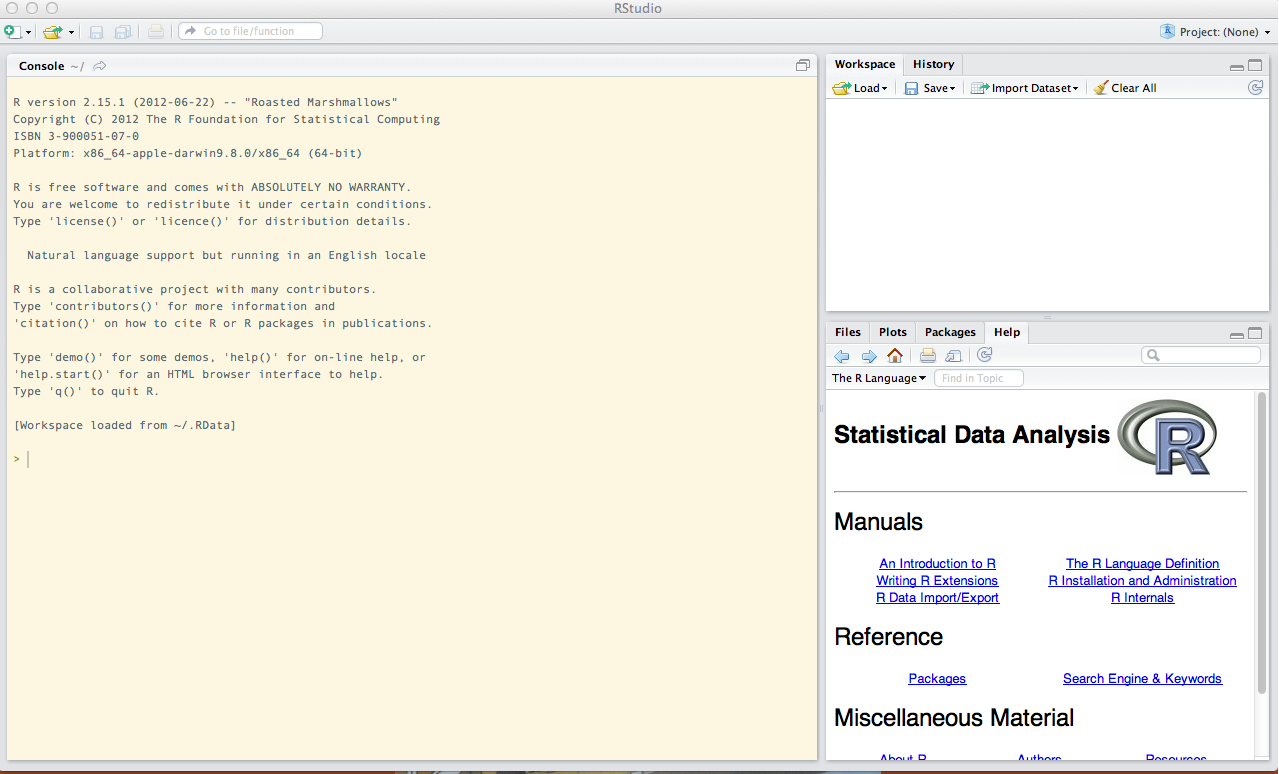
\includegraphics[width = \textwidth]{/git_repositories/Rep-Res-Book/Source/Children/Chapter3/images3/BlankMainPanel.png}
    \end{center}
\end{figure}

In the lower right-hand corner you will see the {\emph{Files/Plots/Packages/Help}} pane. We will discuss the Files pane in more detail in Chapter \ref{DirectoriesChapter}. Basically, it allows you to see and organize your files. The Plots pane is where figures you create in R will appear. This pane allows you to see all of the figures you have created in a session using the right and left arrow icons. It also lets you save the figures in a variety of formats. The Packages pane shows the packages you have installed, allows you to load individual packages by clicking on the dialog box next to them, access their manual files (click on the package name), update the packages, and even install new packages. Finally, the Help pane shows you help files. You can search for help files and search within help files using this pane.  

\paragraph{The source pane}

There is an important pane that does not show up when you open RStudio for the first time. This is the Source pane. The Source pane is where you create, edit, and run your source code files. It also functions as an editor for your markup files. It is the center of reproducible research in RStudio. Let's first look at how to use the Source pane with regular R files. These have the file extension \texttt{.R}.

You can create a new source code document, which will open a new Source pane, by going to \texttt{File} \textrightarrow \: \texttt{New}. In this drop down menu you have the option to create a variety of different source code documents. Select the \texttt{R Source} option. You should now see a new pane with a bar across the top like the first image in Figure \ref{SourcePanes}. To run the R code you have in your source code file simply highlight it\footnote{If you are only running one line of code you don't need to highlight the code, you can simply put your cursor on that line.} and click the \texttt{Run} icon on the top bar. This sends the code to the console where it is executed. The icon next to the right of \texttt{Run} simply runs the code above where you have highlighted. The \texttt{Source} icon next to this runs all of the code in file using R's \texttt{source} command\index{source command}. The icon next to \texttt{Source} is for compiling RStudio notebooks. We will look at creating notebooks later in this chapter.

We will cover how to use the Source pane with literate programming file formats--e.g. R Markdown and R LaTeX--in more detail after first discussing the {\emph{knitr}} basics. 

\begin{figure}[ht]
    \caption{RStudio Source Code Pane Top Bars}
    \label{SourcePanes}
    \begin{center}
    
        \begin{subfigure}
            \caption{R Source Code}
            
\includegraphics[width = \textwidth]{/git_repositories/Rep-Res-Book/Source/Children/Chapter3/images3/RSourceBar.png}
        \end{subfigure}\\[0.5cm]
        
        \begin{subfigure}
            \caption{R Markdown Files}
            
\includegraphics[width = \textwidth]{/git_repositories/Rep-Res-Book/Source/Children/Chapter3/images3/MarkdownSourceBar.png}
        \end{subfigure}\\[0.5cm]
        
        \begin{subfigure}
            \caption{LaTeX Markdown Files}
            
\includegraphics[width = \textwidth]{/git_repositories/Rep-Res-Book/Source/Children/Chapter3/images3/LaTeXSourceBar.png}
        \end{subfigure}
        
    \end{center}
\end{figure}



%%%%%%%%%%%%% Using knitr
\section{Using knitr: the basics}

To get started with {\emph{knitr}}\index{knitr} in R or RStudio we need to learn some of the basic concepts and syntax. The concepts are the same regardless of the markup language that we are using, but much of the syntax varies.

\subsection{File extensions}

When you save a knitable file use a file extension that indicates (a) that it is knitable and (b) what markup language it is using. You can use a number of file extensions for R Markdown files including: \texttt{.Rmd} and \texttt{.Rmarkdown}. LaTeX documents that include {\emph{knitr}} code chunks are generally called R Sweave\index{R Sweave} files and have the file extension {\tt{.Rnw}}. This terminology is a little confusing. It is a holdover from {\emph{knitr}}'s main literate programming predecessor {\emph{Sweave}}.\cite{Leisch2002} You can also use the file extension \texttt{.Rtex}, which is less confusing file extension. However, the code chunk syntax for \texttt{.Rtex} files is different from that use in \texttt{.Rnw} files. We'll look at this in more detail below.

\subsection{Code Chunks}

When we want to include R code into our presentation documents we place them in a code chunk\index{code chunk}. Code chunk syntax differs depending on the markup language we are using to write our documents. Let's see the syntax for R Markdown and R LaTeX files.

\paragraph{R Markdown}

In R Markdown files we begin a code chunk by writing: \`\`\`\ \{r\}. A code chunk is closed--finished--simply with: \`\`\`\. For example:



















